\documentclass[a4paper,titleauthor]{mwart} 

\usepackage{polski}
\usepackage[utf8]{inputenc}
\usepackage{graphicx} %pakiet do wstawiania grafiki
\usepackage[hyphens]{url} %pakiet do wstawiania linkow
%\usepackage[hidelinks,breaklinks]{hyperref}
\usepackage{authblk}%pakiet do tworzenia afiliacji
\usepackage{tabularx}%pakiet do tabel
\usepackage[a4paper, left=2cm, right=2cm, top=3cm, bottom=3cm]{geometry}
\usepackage{listings}
\usepackage{placeins}%pakiet do kontroli umieszczania obiektow
\usepackage{hyperref}%pakiet do m.in. kolorowania linkow

\usepackage[tablegrid,owncaptions]{vhistory}
\renewcommand{\vhhistoryname}{Historia zmian}
\renewcommand{\vhversionname}{Wersja}
\renewcommand{\vhdatename}   {Data}
\renewcommand{\vhauthorname} {Autor}
\renewcommand{\vhchangename} {Opis zmian}

\renewcommand\figurename{Rys.}%skrocony podpis
\renewcommand\lstlistingname{Wydruk}


%------------------------------------------------------------------------
% Dane do strony tytułowej

\title{{\Huge  Projekt SYCYF}\\ - \\{\Large Zespół nr 6}\\ }

\author{Sofiia Levchenko \and Joanna Stalenczyk \and Julia Boryslawska \and Jakub Tarczynski \and Jan Zobniow}

\date{\today}

%------------------------------------------------------------------------
% Początek dokumentu
\begin{document}
	

%Automatycznie generowany tytuł dokumentu
\maketitle
%------------------------------------------------------------------------
% Automatycznie generowany spis treści
\tableofcontents

%------------------------------------------------------------------------
\section{Wstęp}
\label{sec:wstep}%etykieta

Raport bedzie dokumentowany \textbf{przyrostowo} zgodnie z realizacja projektu. Poszczególne etapy realizacji projektu obejmują: 

\renewcommand{\labelenumi}{\Roman{enumi}}
\begin{enumerate}\setlength{\itemsep}{0.2\baselineskip} 
	\item Etap wstępny – stworzenie zespołu i organizacja warsztatu pracy, 
	\item Etap zdobywania informacji – analiza literatury, istniejących metod, zebranie wiedzy teoretycznej związanej z tematem projektu, 
	\item Etap opracowania koncepcji – szukanie rozwiązań, najlepiej sprawdzi się proces burzy mózgów (mapy myśli), opracowanie koncepcji rozwiązania  na podstawie zdobytej wiedzy, opracowanie prostego modelu referencyjnego (Python, MATLAB/GNU Octave, itp) i danych do testowania  
	\item Etap implementacji – na tym etapie rozwijamy i rozbudowujemy koncepcje projektowe docelowego systemu, modelujemy elementy systemu w HDL, weryfikujemy funkcjonalnie, integrujemy i oceniamy prototypy, 
	\item Etap uruchomienia – wdrożenie projektu, uruchomienie na docelowej platformie, przetestowanie według wcześniej opracowanych scenariuszy testowych. 
\end{enumerate}

Prace wykonane w ramach każdego etapu beda opisane w oddzielnych rozdziałach raportu.

\section{Organizacja prac}
\label{sec:organizacja}

Rozdział ten będzie opisywał zadania zrealizowane w ramach Etapu \texttt{I}. W tym rozdziale będą omówione:

\begin{itemize}
	\item analiza podejścia Design Thinking oraz trzech jego wersji (pięć kroków Design Thinkig'u, trzy zachodzące na siebie fazy procesu Design Thinking'u oraz cztero-fazowy proces "Double Dimond")
	\item wybor jedynego sposobu zarządzania projektem
	\item analiza różnego rodzaju narzędzi (TeXstudio, Overleaf, Microsoft Word, Microsoft Teams, Skype, GitHub oraz GitLab)
	\item organizacja warsztatu pracy, dobór narzędzi (Overleaf, Microsoft Teams, GutHub, itp.)
	\item ostateczny dobór narzędzi
	\item organizacja warsztatu pracy
\end{itemize}

\subsection{Design Thinking}
\label{sec:design_thinking}
Co to jest "Design Thinking?" \newline
\newline
Design thinking – jest to proces odnoszący się do procesów poznawczych, strategicznych i praktycznych, dzięki którym koncepcje projektowe (propozycje nowych produktów, usług itp.) są opracowywane przez projektantów i / lub zespoły projektowe~\cite{DesignThinking1}. \newline \newline Wiele osób próbowało sformalizować podstawowe zasady zastosowania myślenia projektowego w organizacjach, za pomocą modeli procesów i metodologii. Pomimo niekończących się modyfikacji i mutacji istnieją trzy, trwałe, ogólne przyjęte modele~\cite{DesignThinking2}:

 \begin{itemize}
 	\item Pięć kroków Design Thinkig'u
 	\item Trzy zachodzące na siebie fazy procesu Design Thinking'u
 	\item Cztero-fazowy proces "Double Dimond"
 \end{itemize}

Diagramy i słownictwo mogą się różnić, ale we wszystkich modelach myślenia projektowego występują wyraźne tematy:

 \begin{itemize}
	\item \textbf{Zorientowane na człowieka}\newline \newline Fazy odkrywania i inspiracji koncentrują się na badaniach proponowanego użytkownika - "Kim oni są?", "Czego chcą / potrzebują?", "Jak się zachowują?" Chodzi o budowanie empatii przez zespół projektowy z użytkownikiem końcowym i zrozumienie, dla kogo projektują.\newline
	\item \textbf{Iteracyjny} \newline \newline Fazy opracowywania, dostarczania i wdrażania skupiają się na usuwaniu najsłabszych pomysłów i ulepszaniu najsilniejszych poprzez prototypowanie, testowanie i optymalizację.\newline
	\item \textbf{Interdyscyplinarne} \newline \newline Wszystkie modele pokazują podróż, która rozbiega się i zbiega, przynajmniej w początkowe rozwiązanie. Każda faza nie jest własnością jednego zespołu z ustalonymi zadaniami; zamiast tego wspólny zespół projektowy wyrusza razem w podróż. Należy zauważyć, że zespoły interdyscyplinarne różnią się od zespołów multidyscyplinarnych tym, że każdy z nich ma wspólną odpowiedzialność za projekt i jego sukces, zamiast opowiadać się za własną specjalizacją.
 \end{itemize}

 \subsubsection{Zalety i wady Design Thinking'u}
Do głównych zalet należą:\newline
\begin{itemize}
\item Ułatwia i przyspiesza przyjęcie rozwiązania: dzięki takiemu podejściu projektowanie oparte na Design Thinking zaczyna się od potrzeby użytkownika końcowego, kończy na zbudowaniu rozwiązania (technologicznego lub procesowego), które jest dla niego naprawdę cenne.
\item Silne zaangażowanie użytkownika końcowego, który czuje się zaangażowany już od strony projektowej: sposób dla firm na ulepszenie swoich pracowników i „wzięcie ich na pokład” stojącego przed nimi wyzwania;
\item Iteracyjne podejście na etapie projektowania pozwala przetestować propozycje rozwiązań i modyfikować je, aż do osiągnięcia najbardziej odpowiedniego rozwiązania przed przystąpieniem do faktycznego wdrożenia;
\end{itemize}
\vspace{0,5cm}
\hspace{0,5cm}Wady Design Thinking'u:\newline
\begin{itemize}
\item Projekt moze trwać długo, a końcową werseję można zastosować tylko do ograniczonych celów
	\item Zastosowanie metodologii projektowania korporacyjnych rozwiązań cyfrowych może kolidować z ograniczeniami nałożonymi przez integrację z już używanymi rozwiazaniami.
	\item Myślenie projektowe wymaga bezpośredniego zaangażowania użytkowników, którzy muszą mieć możliwość wniesienia własnego wkładu (dostępność czasu i zasobów)
\end{itemize}
 

 \subsubsection{Pięć kroków Design Thinkig'u}
 Model ten składa się z 5 etapów: empatyzacji, definiowania problemu, kreatywnego myślenia, tworzenia prototypu, testowania.
\begin{figure}[h]
 	\centering
 	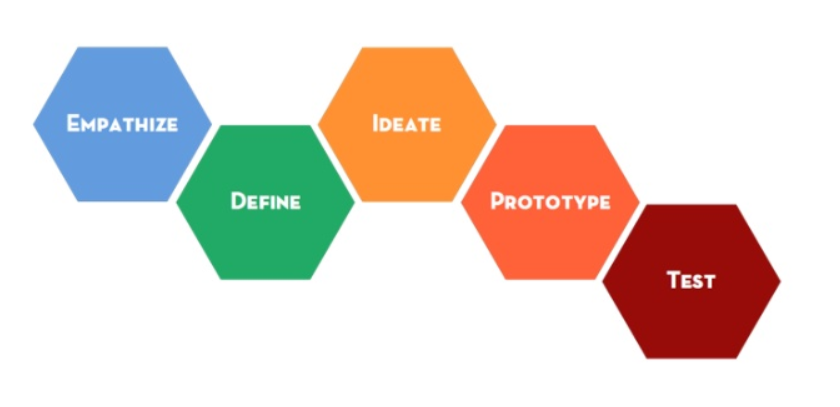
\includegraphics[width=0.8\textwidth]{5krokow.PNG}
 	\caption{Pięć kroków Design Thinkig'u}
 \end{figure}
 \begin{itemize}
     \item \textbf {Empatyzacja}\newline \newline
     W pierwszym kroku skupiamy się na człowieku, czyli odbiorcy naszego projektu. Staramy się zrozumieć czego potrzebuje, dlaczego tego potrzebuje, w jaki sposób będzie z tego korzystał. Robimy to, ponieważ często tworzymy innym, rozwiązujemy cudze problemy, przez co musimy je najpierw dobrze zrozumieć. \newline
     \item \textbf{Definiowanie problemu}\newline \newline
     Gdy już poznamy odbiorcę, naszym zadaniem jest odpowiednie zdefiniowanie problemu, odnalezienie czegoś przydatnego, czegoś co zaspokoi jego potrzeby. Jest to ważny etap, ponieważ od tego zależy nad czym dalej będziemy pracować.\newline \newline
     \item\textbf{Kreatywne myślenie}\newline \newline
     W następnym etapie podchodzimy do problemu jakby nie istniały żadne ograniczenia finansowe ani fizyczne, uruchamiamy kreatywne myślenie. W tym kroku nie zależy nam na odnalezieniu odpowiedniego rozwiązania, tylko na wymyśleniu jak najrozmaitszych pomysłów, co się przyczyni do innowacyjności projektu.\newline
     \item\textbf{Tworzenie prototypu}\newline \newline
     Następnie według tego modelu należy stworzyć prototyp. Powinien on być tani oraz szybki do zrobienia. Jego zadaniem jest ułatwienie wyobrażenia potencjalnych wad, niedociągnięć oraz wywołanie emocji wśród osób testujących, przez co będą w stanie więcej zauważyć, podać konkretniejsze uwagi.\newline
     \item\textbf{Testowanie}\newline \newline
     Ostatni krok polega na przeanalizowaniu wszystkich zdobytych informacji oraz wykorzystaniu ich w trakcie testowania. Osobom testującym należy zapewnić warunki, w których normalnie by korzystały z tego projektu. W tym ostatnim etapie dowiadujemy się jeszcze więcej o użytkowniku. Dzięki testowaniu widzimy czy nasze rozwiązanie jest odpowiednie, co powinniśmy zmienić, a może nawet zacząć proces od początku.
 \end{itemize}


 \subsubsection{Trzy zachodzące na siebie fazy procesu Design Thinking'u}

Drugim w kolejce jest model, który nosi nazwę "Trzech zachodzacąych na siebie faz procesu Design Thinking'u" ~\cite{Proces2}. Jest to proces skupiony głównie na człowieku. \newline \newline 
Co to znaczy? \newline \newline
 Projektowanie zorientowane na człowieku polega na budowaniu głębokiej empatii z ludźmi dla których projektujesz; generowanie tony pomysłów; budowanie wiązki prototypów; dzielenie się tym, co stworzyłeś z odbiorcami i ostatecznie wypuszczenie na rynek nowego, innowacyjnego rozwiązania. \newline \newline
Konstrukcja skoncentrowana na człowieku, w danym procesie, składa się z trzech faz:\newline
 \begin{itemize}
 \item W fazie inspiracji dowiesz się o potrzebach bezpośrednio od ludzi, dla których coś projektujesz, zanurzając się w ich życiu. 
 \item W fazie idei zrozumiesz, czego się nauczyłeś, zidentyfikujesz możliwości projektowania i stworzysz rozwiązania. 
 \item Na etapie wdrażania wprowadzisz swoje rozwiązania w życie, a ostatecznie na rynek. Będziesz wiedział, że Twój projekt odniesie sukces, ponieważ w centrum procesu są ludzie, którym chcesz służyć. \newline \newline
 
\begin{figure}[h]
 	\centering
 	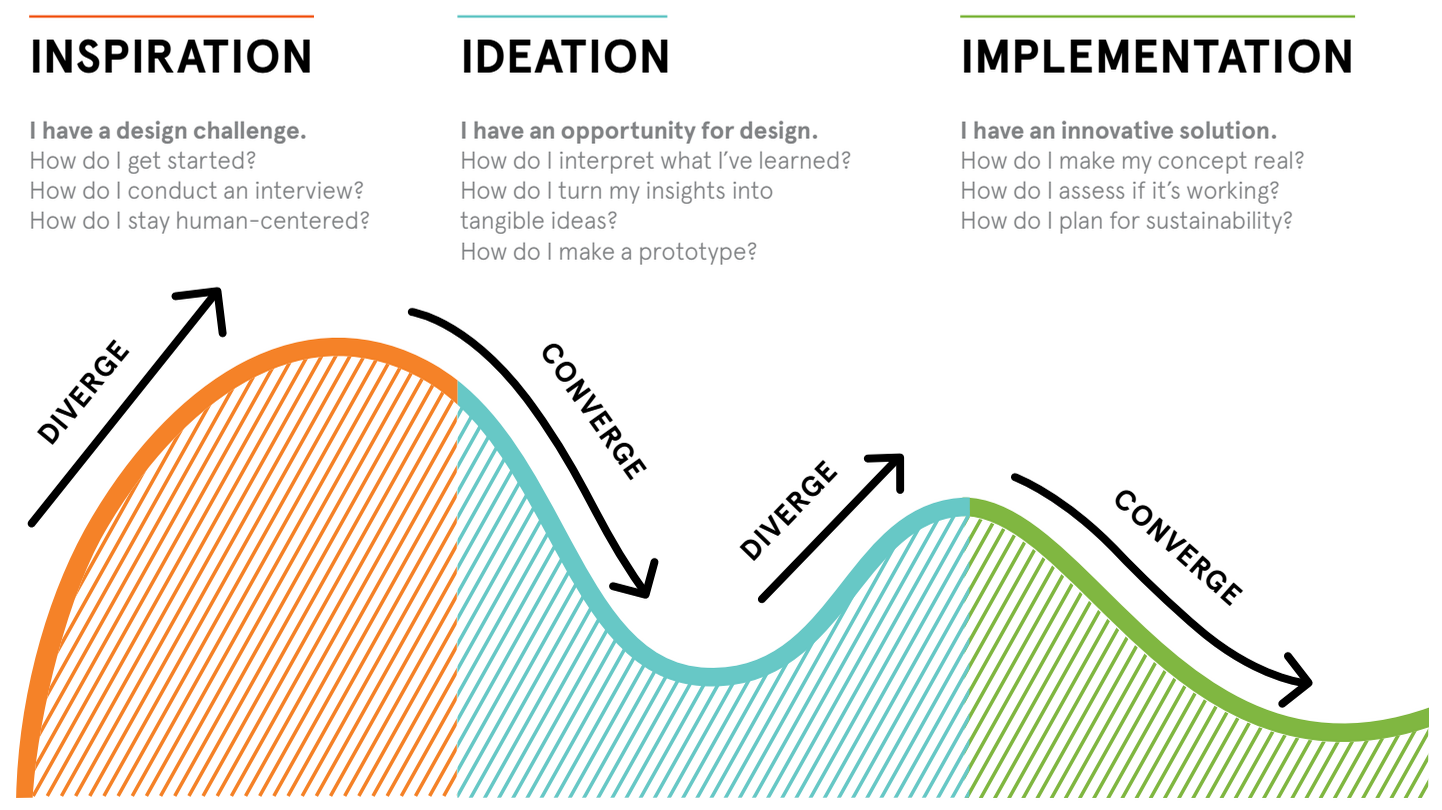
\includegraphics[width=0.6\textwidth]{2}
 	\caption{Trzy zachodzące na siebie fazy procesu Design Thinking'u}
 \end{figure}

\end{itemize}

 
 \subsubsection{Cztero-fazowy proces "Double Dimond"}
 W tym modelu dwa diamenty reprezentują proces zagłębiania problemu, a następnie podejmowanie działań.
  \begin{figure}[h]
 	\centering
 	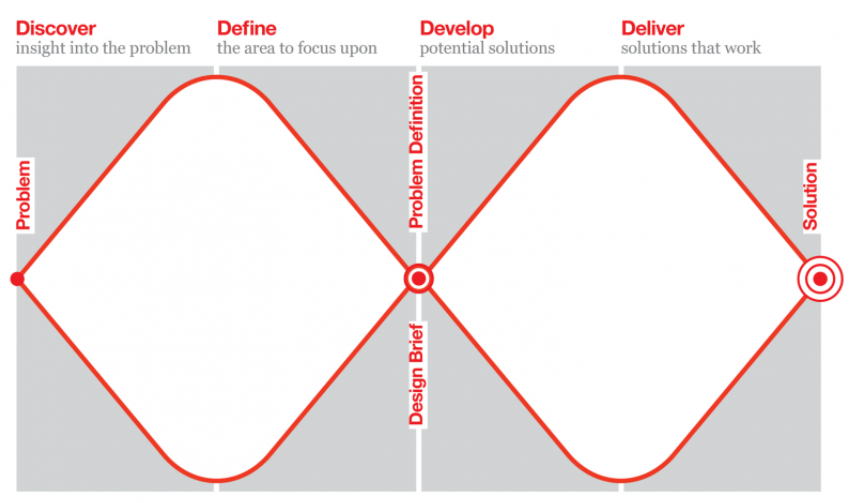
\includegraphics[width=0.6\textwidth]{DoubleDiamond2.PNG}
 	\caption{Cztero-fazowy proces "Double Dimond"}
 \end{figure}
 \begin{itemize}
     \item \textbf{Pierwszy diament}\newline \newline
     Odkrywanie – pomaga zrozumieć problem, a nie tylko założyć jaki on jest. Etap ten wiąże się z rozmawianiem oraz poznawaniem ludzi, których ten problem dotyczy.\newline
     Definiowanie - Informacje zebrane z fazy odkrywania mogą pomóc w zdefiniowaniu wyzwania w inny sposób.\newline
     \item\textbf{Drugi diament}\newline \newline
     Rozwój - zachęca ludzi do udzielania różnych odpowiedzi na jasno zdefiniowany problem, szukania inspiracji z innych źródeł i wspólnego projektowania z szeregiem różnych osób.\newline
     Dostarczanie - obejmuje testowanie różnych rozwiązań na małą skalę, odrzucanie tych, które nie będą działać oraz ulepszanie tych, które mają potencjał.\newline

 
 \end{itemize}

\subsection{Zarządzanie projektem}
\label{sec:zarządzanie_projektem}

\subsubsection{Metody}
\label{sec:narzędzia}
Po analizie wszystkich trzech modeli Design Thinking'u, zdecydowaliśmy się, na podążanie za jedną z metod - Double Diamond. Jest to najbardziej korzystny model w przypadku problememu, z jakim się zetkneliśmy. W tym celu dokładnie zapoznamy się z danym zadaniem, spróbujemy spojrzeć na problem z wielu perspektyw, weźmiemy pod uwagę pomysły i rozwiązania zaproponowane przez każdego członka zespołu. Przanalizujemy oraz wypróbujemy wszystkie możliwości, by finalnie dotrzeć do najbardziej korzystnego rezultatu. 

\vspace{1cm}
\subsubsection{Narzędzia}
\label{sec:narzędzia}


Dostępnych jest wiele narzędzi, które ułatwiają komunikację, usystematyzowanie oraz koordynowanie pracy grupowej. W tym podrozdziale przedstawimy niektóre aplikacje, z którymi można zetknąć się podejmując się wykonywania projektów zespołowych, by następnie dokonać wyboru najbardziej korzystnych w działaniu dla nas narzędzi. \newline \newline

\fbox{Programy do obróbki tekstu:} \newline 

\textbf{LaTeX} \newline
\indent

Zalety:
\begin{itemize}

\item[-]
Wszystkie tytuły sekcji / podpisy tabel, grafik, wykresów są jednakowo formatowane;

\item[-]
Program generuje spis treści;

\item[-]
Pliki PDF generowane przy pomocy LaTeX-a są estetyczne wizualnie;

\item[-]
Możliwość tworzenia wykresów/diagramów za pomocą kodu, bez używania dodatkowych programów; 

\item[-]
LaTeX jest programem o wolnym dostępie – nie musimy za niego płacić;

\item[-]
Pliki LaTeX-a możemy otwierać przy pomocy wielu narzędzi. Możemy używać programów zainstalowanych na komputerze lub wykorzystywać programy internetowe. W przypadku tych drugich istnieje możliwość dzielenia projektu między wiele osób. 
\end{itemize}

\indent

Wady:
\begin{itemize}


\item[-]
Konieczność stosowania odpowiednich bibliotek;

\item[-]
Trudniejsza zmiana np. rodzaju czcionki, marginesów i innych parametrów formatowania pliku w porównaniu do narzędzi typu Word;

\item[-]
Aby korzystać z LaTeX-a trzeba nauczyć się odpowiednich komend oraz poznać składnię.
\end{itemize}

\vspace{1cm}
\textbf{Microsoft Word:}

\indent

Zalety:
\begin{itemize}

\item[-]
Program nie wymaga poznania specjalistycznej składni ani komend;
\item[-]
W łatwy sposób można zmienić parametry np. czcionki, marginesów;
\item[-]
Nie wymaga importowania odpowiednich bibliotek.
\end{itemize}

\indent

Wady:
\begin{itemize}

\item[-]
Wprowadzenie zapisów (symboli) matematycznych jest bardzo trudne;
\item[-]
 Występują problemy z formatowaniem (np. odpowiednie marginesy, akapity);
\item[-]
Podczas przesyłania pliku zdarza się jego deformacja.
\end{itemize}

------------------------------------------------------------\newline \newline
\fbox{Aplikacje komunikacyjne:} \newline 

\textbf{Microsoft Teams} \newline
\indent

Zalety:
\begin{itemize}

\item[-]
Umożliwa komunikację telefoniczną oraz multimedialną, rejestrowanie rozmów ;

\item[-]
Oferuje integracje z duża liczbą innych usług(Word, Excel, Planner, Outlook);

\item[-]
Darmowy dostęp;


\end{itemize}

\indent

Wady:
\begin{itemize}

\item[-]
Mało intuicyjny sposób użytkowania;
\end{itemize}
\vspace{0,8cm}

\textbf{Slack} \newline
\indent

Zalety:
\begin{itemize}

\item[-]
Umożliwa komunikację telefoniczną oraz multimedialną, rejestrowanie rozmów ;

\item[-]
Oferuje integracje z duża liczbą innych usług(Word, Excel, Planner, Outlook);

\item[-]
Darmowy dostęp;


\end{itemize}

\indent

Wady:
\begin{itemize}

\item[-]
Mało intuicyjny sposób użytkowania;
\end{itemize}

\vspace{0,8cm}
\textbf{Skype} \newline
\indent

Zalety:
\begin{itemize}

\item[-]
Umożliwa wykonywanie połączeń telefonicznych oraz video rozmów;

\item[-]
Możliwość udostępniania ekranu rozmówcy;

\end{itemize}

\indent

Wady:
\begin{itemize}

\item[-]
Do korzystania z opcji videokonferencji, która w naszym przypadku jest kluczowa - wymagane wykupienie subskrybcji premium;

\item[-]
Brak połączenia narzędzia z innymi aplikacjami, służącymi do organizacji pracy.
\end{itemize}
------------------------------------------------------------\newline \newline
\fbox{Organizacja pracy:} \newline 

\textbf{Trello} \newline
\indent

Zalety:
\begin{itemize}

\item[-]
Umożliwa wizualne przechowywanie zasobów oraz aktualizowanie na bieżąco dokumentacji ;

\item[-]
Możliwość udostępniania członkom zespołu postępów pracy;

\item[-]
Liczne opcje formatowania tablic;


\end{itemize}
\vspace{1cm}

\textbf{GitHub} \newline
\indent

Zalety:
\begin{itemize}
\item[-]
Kontrola wersji;
	
\item[-]
Struktura branchowa;
	
\item[-]
Miejsce na hosting plików;
	
\item[-]
Możliwość zastosowania w przyszłej karierze zawodowej;
	

Wady:
\item[-]
Wymagane nauczenie się działania systemu
	
\item[-]
Poznanie składni komend
\end{itemize}

------------------------------------------------------------\newline \newline \newline \newline
\vspace{0,5cm}
\textbf{WNIOSKI} \newline

Po analizie wad i zalet powyższych programów oraz aplikacji doszliśmy do następujących wniosków: \newline
Głównym narzędziem służącym do sporządzania sprawozdań będzie \textbf{LaTeX}. Jest to dla naszego zespołu najbardziej korzystny wybór z uwagi na możliwość edycji tekstu przez każdego z członków grupy, w tym samym momencie. W ten sposób możemy dzielić projekt między wszystkimi. Oprócz tego dokument tworzony w LeTeXu wygląda schludnie i estetycznie, nie ulega on formatowaniu na różnych urządzeniach, z których korzystamy. 
Do komunikacji będzie służyła nam aplikacja \textbf{Microsoft Teams}. Główną oraz kluczową w wyborze zaletą, jest możliwość tworzenia telefonicznych konferencji, a także opcja połączenia pracy MSTeams z systemem Git oraz Trello.
Oprócz MSTeams w nagłych i pilnych sytuacjach korzystamy z aplikacji \textbf{Messenger}, która jest w tym momencie najszybszą formą komunikacji. 
Kolejnym narzędziem, które wybraliśmy jest wcześniej wspomniany system kontroli wersji - \textbf{Git}, na platformie github.com.
Będzie służył nam głównie do systematycznej akutalizacji dokumentów oraz możliwości przekazywawnia ich między członkami zespołu. 
Dzięki aplikacji \textbf{Trello} nasza praca pozostanie odpowiednio skoordynowana, a możliwość połączenia aplikacji z Microsoft Teams i otrzymywaniu w ten sposób powiadomień, sprawi, że każdy z członków zespołu wykona dane mu zadanie w odpowiednim czasie. 

\section{Informacje podstawowe}
\label{sec:informacje_podstawowe} 
Rozdział ten będzie opisywał zadania zrealizowane w ramach Etapu \texttt{II}. W tym rozdziale będą omówione:\newline 
\begin{itemize}
	\item opis zadania projektowego 
	\item ogólne wiadomości o steganogarfii, strukturze steganologii oraz przykładowy model systemu steganograficznego
	\item wspólczesne metody steganograficzne
	\item metody cyfrowego przetwarzania sygnalow stosowane w dzwieku
	\item analiza wybranych metod cyfrowego przetwarzania sygnałow w steganografii sygnałow dzwiekowych
	\item narzędzia, oprogramowanie wykorzystywane przy analizie sygnałów cyfrowych
	\item wnioski
	\end{itemize} 
\subsection{Zadanie projektowe}

Głównym zadaniem tego projektu jest wykrycie tajemniczej wiadomości "z kosmosu" zakodowanej niewadomym sposobem w sygnalie dzwiękowym. Do dyspozycji mamy trzy pliki dzwiękowe formatu ".wav" oraz plik tekstowy z niektórą ilością próbek danego cyfrowego sygnału. \newline  \newline 

\subsection{Steganografia}

Steganografia - jest to nauka zajmująca się ochroną cennej informacji poprzez jej ukrywanie w innej nie mającej wartości. Do ukrywania danych zaczęto wykorzystywać sygnał w postaci cyfrowej. \newline Jeśli adwersarz nie będzie świadomy faktu istnienia ukrytej informacji, lub nie będzie znał miejsca jej ukrycia, to nie będzie w stanie jej odczytać. \newline \newline 
Dalej zapoznamy się z tą nauką trochę bliżej, oraz przeanalizujemy metody cyfrowego przetwarzania sygnałów pod kątem ich przydatności w steganografii komputerowej, wykorzystującej dźwięk jako kontener.

\subsubsection{Steganologia i jej struktura}
 \begin{itemize}
	\item \textbf {Steganologia - z czego się składa?}\newline \newline
Steganologia obejmuje dwie dziedziny – steganografię zajmującą się ochroną informacji oraz przeciwstawną do niej steganoanalizę. Celem tej nauki jest ochrona informacji.\newline \newline  Steganologia nie dokonuje przekształceń informacji lecz zajmuje się ukrywaniem jej istnienia, tak by osoby postronne nie były w stanie stwierdzić jej istnienia.\newline \newline  Obecnie najczęściej wykorzystywana jest postać cyfrowa sygnału dźwiękowego a on sam przekazywany i przetwarzany jest w tej właśnie postaci. Występuje tu zjawisko uniezależnienia danych od nośnika. Będziemy dalej opracowywać metody powiązane bezpośrednio z danymi cyfrowymi.

	\item \textbf {Struktura steganologii}\newline \newline
	
	Jak było już omówione, steganologia obejmuje dwie dziedziny: steganografię i stegoanalizę.\newline \newline
	\textbf{Steganografia} zajmuje się ukrywaniem cennej informacji w innych danych nie mających wartości, tak by osoba postronna nie była w stanie wykryć istnienia dodatkowych danych. Dokonuje się tego poprzez wprowadzenie do oryginalnego nośnika niewielkich zmian, których ludzkie zmysły nie są w stanie wykryć. Istotne jest również zachowanie poprawnej wartości wszystkich parametrów, które mogą zostać zbadane podczas analizy sygnału. \newline \newline
	\textbf{Steganoanaliza} zajmuje się wykrywaniem ukrytych informacji oraz ich odczytywaniem lub niszczeniem. \newline Możliwe jest to dzięki wnikliwej analizie nośników i badaniu ich parametrów. W przypadku gdy znacznie odbiegają one od spodziewanej wartości sygnał poddawany jest szczegółowej analizie ze względu na duże prawdopodobieństwo istnienia w nim ukrytych danych. \newline
 \end{itemize}

\subsubsection{Model systemu steganograficznego}

Przykładowy model systemu steganograficznego zaprezentowany został na rysunku niżej.

  \begin{figure}[h]
	\centering
	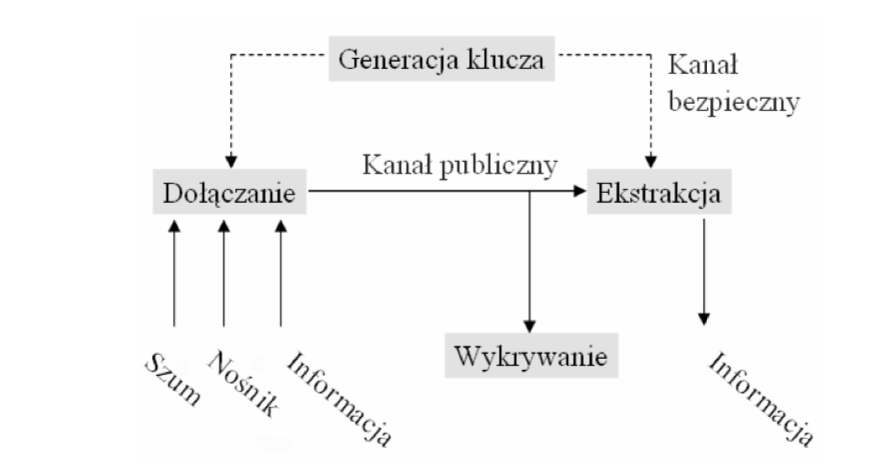
\includegraphics[width=0.6\textwidth]{model}
	\caption{Przykładowy model systemu steganograficznego}
\end{figure}

Przy komunikacji strony muszą uzgodnicz klucz steganograficzny, z którego będą korzystać, musi on zostać dostarczony w sposób bezpieczny, tak by przeciwnik nie miał możliwości zdobycia go. Gwarantuje on bezpieczeństwo systemu. Mając uzgodniony klucz nadawca dołącza za jego pomoca informację do kontenera. Często jest ona wcześniej szyfrowana. Niekiedy jednocześnie z informacją dołączany jest dodatkowy szum, który ma za zadanie dodatkowo utrudnić detekcję właściwej informacji. Przygotowany stegokontener jest przesyłany kanałem publicznym do odbiorcy, który za pomocą klucza odczytuje z niego dołączoną informację. Działanie takiego systemu polega na "grze" pomiędzy trzema graczami. Dwaj z nich porozumiewają się przesyłając kanałem publicznym informacje ukryte w innym nośniku. Trzeci z nich próbuje wykryć, która część przesyłanych danych zawiera utajnioną informację. Jeśli mu się to uda przystępuje do wyodrębniania wiadomości z nośnika. My w takim modelu występujemy tym trzecim graczem, który chcę zdobyć ukrytą informację.

\subsection{Metody steganograficzne}

Metod stegonograficznych istnieje dużo i w naszym czasie ilość ich rośnie. Ale chcemy na tym etapie skupić się na kilku z nich, a same: \newline
\begin{itemize}
\item dodawanie echa
\item filtrowanie
\item metoda najmniej znaczacego bitu
\item modyfikacja szumu
\item maskowanie rownoczesne i czasowe
\item zmiana czestotliwosci probkowania 
\item modulacja
\item rozpraszanie widma
\end{itemize}
\subsubsection{Dodawanie echa}
Echo - jest to odbicie dźwięku, które dociera do słuchacza z opóźnieniem po dźwięku bezpośredniego.
\newline\newline
Ludzkie ucho nie potrafi odróżnić echo z oryginalnym dźwiękiem bezpośrednim, jeśli opóźnienie wynosi mniej niż 2 milisekundy a siła go nie przekracza 0.4 amplitudy dźwięku oryginalnego po sygnale lub też bezpośrednio przed nim.
\newline\newline
Dlatego czasem wykorzystują to zjawisko do ukrycia dodatkowej informacji. Ukrywanie danych odbywa się za pomocą sterowalnego filtru opóźniającego, którego zadaniem jest dodanie do oryginalnego sygnału jego kopii opóźnionego o zadany czas. 
\newline\newline

  \begin{figure}[h]
	\centering
	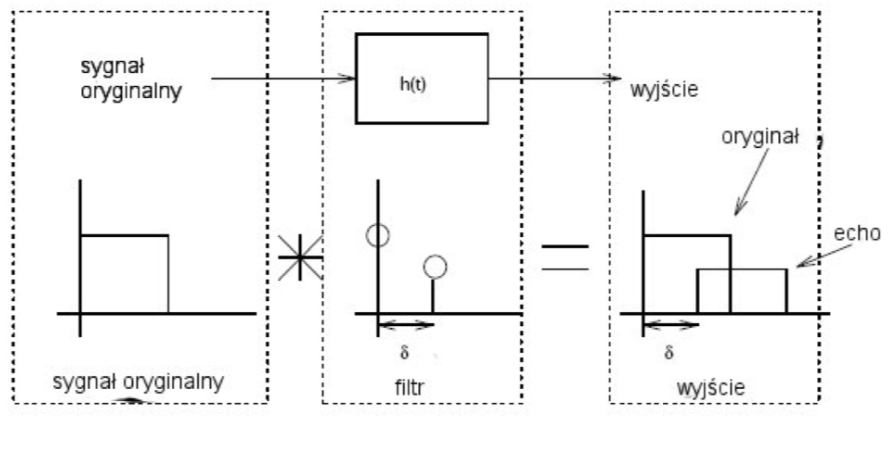
\includegraphics[width=0.4\textwidth]{echo}
	\caption{Przykładowy model systemu steganograficznego}
\end{figure}

Taką metodą można dodawać ukryte wiadomości w postaci binarnej, gdzie 0 oraz 1 występują echami o różnej amplitudzie lub opróżnieniu. Także stosowaną jest metoda dodawania pre-echa (sygnał echa jest dodawany przed właściwym sygnałem) jako wartości logicznej zera, oraz echa po sygnale jako wartości logicznej 1. 
\newline\newline

\subsubsection{Filtrowanie}

Filtr cyfrowy - to jest system, który wykonuje operacje arytmetyczne na próbkach dyskretnego sygnału w celu zmniejszenia lub zwiększenia pewnych aspektów tego sygnału
\newline\newline
Filtracja - proces przetwarzania dokonywany na sygnale w dziedzinie czasu, powodujący zmiany w widmie sygnału oryginalnego. Zmiana polega na redukcji (odfiltrowaniu) pewnych niepożądanych składowych sygnału wejściowego - zatem filtr przepuszcza pewne częstotliwości, tłumiąc inne. Więc, filtry są istotnym narzędziem do wyczyszczenia sygnału od szumu. Niżej jest rzedstawiono schematycznie proces filtracji cyfrowej.
\newline\newline

\begin{figure}[ht]
	\centering
	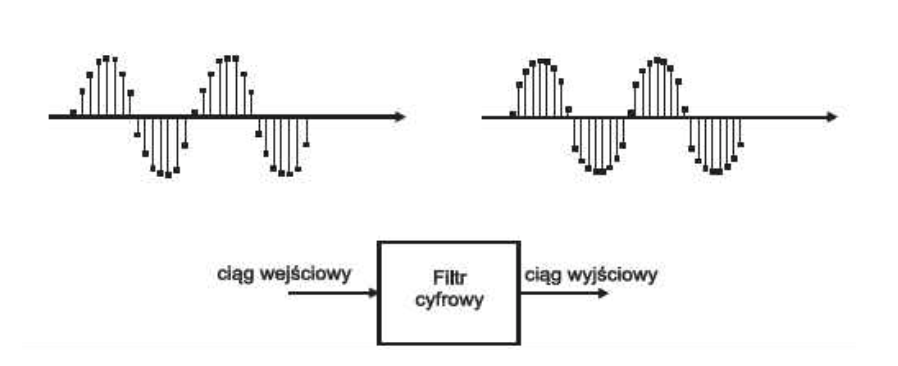
\includegraphics[width=0.5\textwidth]{filter}
	\caption{Schemat procesu filtracji cyfrowej}
\end{figure}

Filtr cyfrowy przetwarza ciąg wartości próbek dyskretnych i jest dedykowany pewnym systemem cyfrowym. Do obliczenia wartości próbek wyjściowych, czyli aby dokonać filtracji, filtr korzysta z dodawania, w podobny sposób jak to się dzieje w procesie uśredniania. 
\newline\newline
Filtr jako taki może być dolno- lub górnoprzepustowy, bądź pasmowy, a poza tym może mieć różne częstotliwości graniczne.
\newline\newline
Tradycyjne filtry liniowe są zwykle oparte na tłumienie.
Wiele filtrów cyfrowych w oparte są na szybkiej transformacie Fouriera, pozwalając manipulować widmem przed konwersją zmodyfikowanego widma z powrotem na sygnał czasu z serii operacji odwrotnej FFT. Filtry te dają O (n log n) koszty obliczeniowe, natomiast inne filtry cyfrowe są zwykle O (n2 ).\newline\newline

\subsubsection{Metoda najmniej znaczącego bitu (Least Significant Bit, LSB)}

Metoda skupiając się na sposobie zakodowania plików źródłowych (.wav) sygnału. W tym sposobie analizowane są wartości ostatnich bitów, każdego z bajtów w pliku binarnym. Jest to powszechny sposób niskopoziomowego ukrycia wiadomości, stosowany w Steganografii.
\newline \newline
Pliki te we wglądzie hexdump wyglądają następująco:

\begin{figure}[ht]
	\centering
	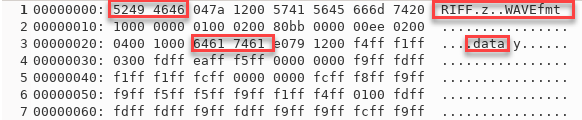
\includegraphics[width=0.8\textwidth]{hexdump.PNG}
	\caption{Hexdump}
\end{figure}

Następnie z odczytano kolejno chunków danych (zaznaczone kolorem czerwonym), możemy sprawdzić wartości ostatnich bitów. Algorytmy stosowane w metodzie LSB podążają daną sekwencją kodując wiadomość z określonym cyklem np. co 2,3 chunk. Znajdując sekwencje poprzez Wczytanie tych ostatnich wartości jesteśmy wtedy wstanie odtworzyć ukrytą zawartość.\newline\newline

\subsubsection{Modyfikacja szumu}

Sygnał jaki otrzymaliśmy do zbadania przypomina biały szum.\newline \newline
Kierując się tą informacją postanowiliśmy poszukać metod, które pozwoliłyby na redukcje szumu oraz ustabilizowanie ścieżki dźwiękowej – w efekcie – usłyszenie zaszyfrowanej wiadomości. 
\newline \newline
Jedną z metod przetwarzania sygnału jest właśnie modyfikacja szumu, czyli zastosowanie sygnału zwanego DITHER (do tej pory nie posiada on polskiej nazwy). Polega on na eliminacji szumu poprzez dodanie do sygnału… szumu. Ściślej mówiąc jest to losowy szum, dodawany do sygnału wejściowego. W efekcie otrzymujemy inny szum, słyszalny jako bardzo ciche syczenie.\newline \newline
Pozornie nie jest to tylko usuwanie jednego szumu i zamienienie do drugim. Główną konsekwencją zastosowania sygnału DITHER jest lepsza słyszalność naszego pierwotnego sygnału. Dzieje się tak, ponieważ do szumu białego jesteśmy przyzwyczajeni, gdyż otacza nas on wszędzie na co dzień, więc jego słyszalność jest mniej zauważalna. Do tego należy wziąć pod uwagę, że uzyskany sygnał jest „odfiltrowywany” a poza tym stosuje się uśrednianie. 
\newline \newline
Działanie tej metody przedstawia rysunek: 

\begin{figure}[h]
	\centering
	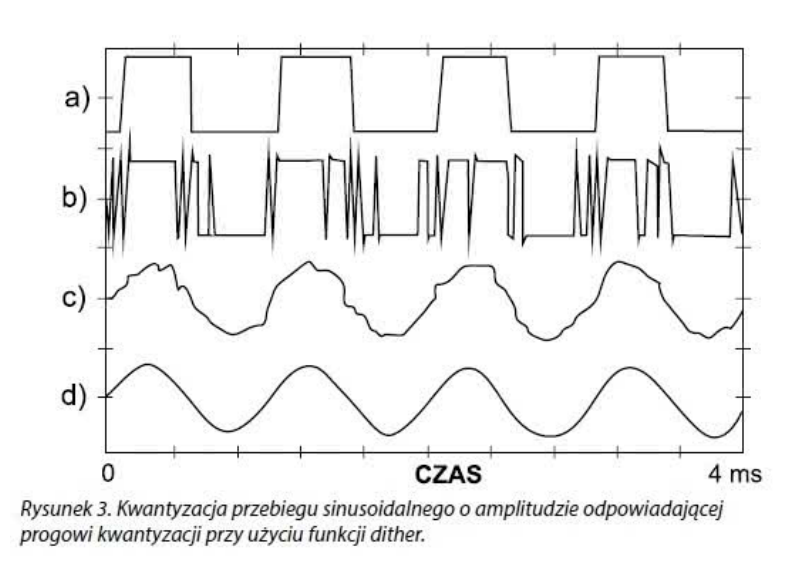
\includegraphics[width=0.7\textwidth]{dither}
\end{figure}

Pierwszy przebieg (a) to sygnał sinusoidalny bezpośrednio po kwantyzacji. Jeżeli jednak dodamy do sygnału oryginalnego dither i skwantujemy taki sygnał, otrzymamy takie „dziwadło”, jak na drugim rysunku (b). \newline \newline
Fakt, że niewiele ma on wspólnego ani z sinusoidą, ani z prostokątem, ani z żadnym innym „normalnym” przebiegiem. Jeżeli jednak zastosujemy uśrednianie w czasie 32 okresów, otrzymamy nieco „pogryziony” przebieg, który jednakże już bardziej przypomina sinusoidę, a po uśrednieniu w czasie 960 okresów nasz sygnał wygląda niemalże jak idealna sinusoida.   


\subsubsection{Maskowanie równoczesne i czasowe}

\textbf{Maskowanie równoczesne} – efekt psychoakustyczny, które polega na zagłuszaniu dźwięków przez inne dźwięki. Zjawisko to polega na tym, że w zależności od natężeń i częstotliwości dźwięków, pewne tony stają się niesłyszalne, podczas gdy w sąsiedztwie występują inne dźwięki. Sygnał maskujący nazywamy maskerem. \newline \newline
 Efekty maskowania służą do eliminowania szumów w sygnale. Gdy ustawimy odpowiedni próg maskowania, sygnał użyteczny może zamaskować szum.
\newline \newline
\textbf{Maskowanie nierównoczesne (czasowe)} – efekt psychoakustyczny, który polega na zagłuszaniu pewnych dźwięków przez inne dźwięki. \newline \newline
W odróżnieniu od maskowania równoczesnego, dźwięk maskujący i dźwięk zamaskowany nie występują w tym samym czasie. Kiedy dźwięk cichszy występuje do kilkunastu sekund wcześniej niż dźwięk głośniejszy (do kilkunastu ms) mamy do czynienia z premaskowaniem (maskowanie wstecz). Zjawisko to zachodzi dzięki temu, że układ słuchowy szybciej przetwarza dźwięki głośniejsze, dzięki czemu może zamaskować wcześniejszy, cichszy dźwięk. Istnieje także maskowanie wprzód (postmaskowanie), które zależy od głośności i czasu trwania tonu maskującego. Postmarkowanie może występować, kiedy głośniejszy dźwięk występuje do kilkuset ms przed dźwiękiem cichszym.

\subsubsection{Zmiana częstotliwości próbkowania}

Podczas cyfrowego nagrywania sygnału dźwiękowego pochodzącego ze źródła analogowego częstotliwość próbkowania oznacza odstępy czasu między kolejnymi próbkami. Im większa jest jej wartość, tym mniej traci się z pierwotnego materiału audio. Aby dołączyć do sygnału dodatkowe dane wystarczy zmodyfikować sygnał rozpraszający zgodnie z przyjętymi założeniami a następnie przy jego pomocy spróbkować oryginalne nagranie. Taką techniką mógł zostać przetworzony badany przez nas sygnał. 

\subsubsection{Modulacja}

W procesie modulacji sygnał informacyjny zostaje skojarzony z pewnym parametrem sygnału dużej częstotliwości, tzw. fali nośną.\newline \newline
Wyróżnianych jest wiele typów modulacji, my jednak skupiliśmy się na tych rodzajach, które mogłyby być użyte do zmodyfikowania badanego przez nas sygnału: 

\begin{itemize}
\item \textbf{Modulacja amplitudy:}\newline \newline Najprostszym przykładem modulacji amplitudy jest dwustanowa modulacja OOK (On-Off Keying), która polega na włączaniu i wyłączaniu sygnału nośnej. Jest to elementarna forma modulacji cyfrowej. W podstawowej postaci modulacji amplitudy obwiednia sygnału nośnej odzwierciedla zmiany sygnału informacyjnego. \newline \newline
\item \textbf{Modulacja częstotliwości:} \newline \newline
1)	W modulacji FM częstotliwość fali nośnej zmienia się pod wpływem sygnału informacyjnego. Proces demodulacji sygnału zmodulowanego częstotliwościowo wymaga zamiany jej na modulację amplitudy przy wykorzystaniu obwodu rezonansowego, który pozwala na uzależnienie sygnału wyjściowego od zmian częstotliwości sygnału zmodulowanego. 

\begin{figure}[h]
	\centering
	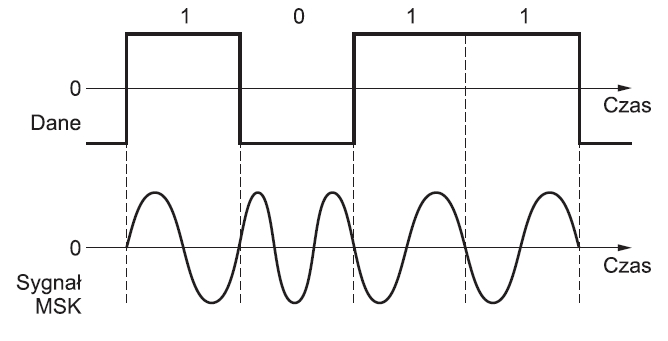
\includegraphics[width=0.7\textwidth]{modulacja1.jpg}
\end{figure}

2)	Przykładem częstotliwości jest również FSK (Frequency Shift Keying). Częstotliwość nośnej w tym wypadku przyjmuje zamiennie dwie wartości, które reprezentują stany logiczne 0 i 1. W ten sposób można zrealizować transmisję ciągu bitów informacyjnych. 
\end{itemize}

\subsubsection{Rozpraszanie widma}
Istotą metod transmisji z rozpraszaniem widma jest nadawanie sygnału w szerokim paśmie częstotliwości, przy poziomie sygnału znacznie poniżej poziomu szumów. \newline \newline
Połączenie tych dwóch właściwości sygnału pozwala osiągnąć założoną przepustowość kanału oraz jednocześnie powoduje, że sygnał taki trudno jest wykryć. 

\subsection{Cyfrowe przetwarzania sygnałów dzwiekowych}

W poprzednim podrozdziale zapoznaliśmy się z metodami \textbf{ukrywania} informacji w sygnalie cyfrowym, ale co zrobić, jeżeli powinniśmy dokonać odwrotnej operacji, nie znając dokładnie \textbf{jak} informacja została zakodowana?\newline \newline
W takim przypadku zwracamy się do cyfrowego przetwarzania sygnałów (w naszym przypadku dzwiękowym) którego zadanie polega na analizie cyfrowego sygnału (w naszym przypadku analizie widmowej).\newline \newline
Dziedzina cyfrowego przetwarzania sygnałów zawiera wiele dobrze opracowanych teoretycznie metod operujących na cyfrowej postaci sygnału dźwiękowego. W niniejszym podrozdziale został przedstawiony krótki przegląd najpopularniejszych metod przetwarzania sygnałów:

\begin{itemize}
	\item transformacja Fouriera
	\item filtrowanie (zasady i struktura są takie same jako w steganografii)
	\item transformacja falkowa
	\item transformacja Gabora
	\item analiza cepstralna
\end{itemize}	

\subsubsection{Transformacja Fouriera}

\textbf{DFT (Dyskretna Transformata Fouriera)} - jedna z najbardziej popularnych i najbardziej wydajnych procedur spotykanych w dziedzinie cyfrowego przetwarzania sygnałów.\newline \newline
 Pozwala ona analizować sygnały w sposób niemożliwy w przypadku sygnałów analogowych. Jest to procedura matematyczna, używana do wyznaczenia zawartości harmonicznej lub częstotliwościowej sygnału dyskretnego (zbiór wartości otrzymany w wyniku próbkowania w dziedzinie czasu sygnału ciągłego).\newline \newline
 Podstawą obliczeń jest ciągłe przekształcenie Fouriera, zdefiniowane następująco:\newline
	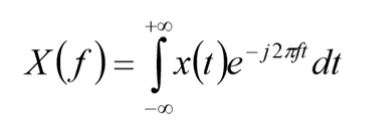
\includegraphics[width=0.3\textwidth]{fourier1}

, gdzie x(n) jest dyskretnym ciągiem spróbkowanych wartości w dziedzinie czasu.\newline\newline
Przy pomocy powyższego równania, funkcję x(t) ciągłą w dziedzinie czasu możemy przetworzyć na funkcję X(f) ciągłą w dziedzinie częstotliwości. Dzięki temu możemy przenieść nasz sygnał z dziedziny czasu do dziedziny częstotliwości, tj. wyznaczyć jego widmo w postaci ciągłej. Umożliwia nam to odczytanie zawartości częstotliwościowej naszego sygnału.
\newline\newline
Wraz z rozwojem technologii i nadejściem komputera, cały dorobek matematyczny w dziedzinie przetwarzania sygnałów, doprowadził do zdefiniowania DFT jako dyskretnego ciągu X(m) w dziedzinie częstotliwości, określonego równaniem:
\newline
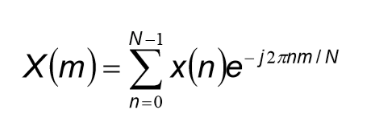
\includegraphics[width=0.3\textwidth]{fourier2}

, gdzie x(n) jest dyskretnym ciągiem spróbkowanych wartości w dziedzinie czasu. \newline\newline
Wartość X(0) w dziedzinie częstotliwości określa składową stałą w widmie sygnału x(n).
Z zależności Eulera wynika, że powyższe równanie jest równoważne z: 
\newline
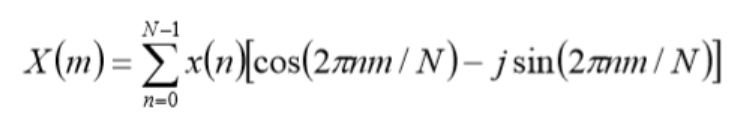
\includegraphics[width=0.6\textwidth]{fourier3}

Powyższy wzór nazywany jest równaniem DFT, dla którego:

\begin{itemize}
\item X(m)  odpowiada m-tej składowej wyjściowej DFT, tj. X(0), X(l), X(2), X(3) itd.;
\item m  indeksowi próbek wyjściowych DFT w dziedzinie częstotliwości, m =0, 1, 2, 3, ..., N-1 
\item x(n)  ciągowi próbek wejściowych, x(0), x(l), x(2), x(3) itd.. 
\item n  indeksowi próbek wejściowych w dziedzinie czasu, n= 0, 1,2,3,...,N-1 
\item N  liczbie próbek ciągu wejściowego oraz liczbie punktów częstotliwości w ciągu wyjściowym DFT.
\end{itemize}
Każdy człon wyjściowy X(m) DFT stanowi sumę punkt po punkcie iloczynu ciągu wartości wejściowego sygnału i przebiegu zespolonego postaci cos(g) – jsin(g).
\newline\newline
Wartość X(0) w dziedzinie częstotliwości określa składową stałą w widmie sygnału x(n). Gdy X(0) nie jest równa zero, to znaczy że ciąg x(n) jest przesunięty o składową stałą i ma pewną niezerową wartość średnią.
\newline\newline
Jeśli DFT potraktujemy jako „czarną skrzynkę”, to miałaby ona następujące właściwości: sygnały wchodzące i wychodzące są sygnałami dyskretnymi oraz liczba próbek wchodzących do procesu jest równa liczbie próbek z niego wychodzących.
\newline\newline

\textbf{Przykład DFT}
   \begin{figure}[ht]
    	\centering
    	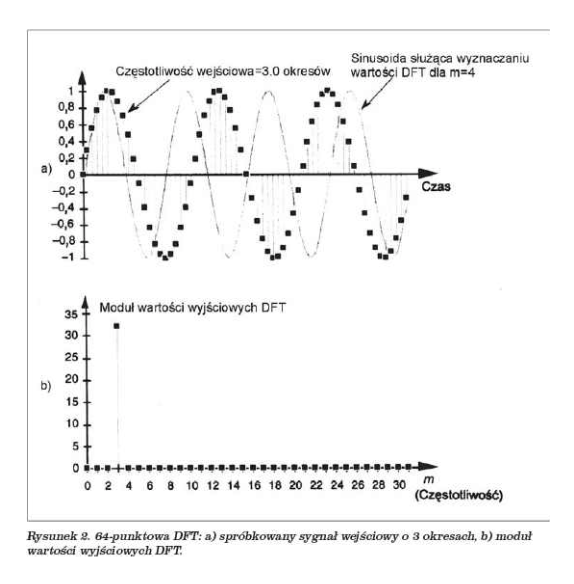
\includegraphics[width=0.6\textwidth]{fourier4}
   \end{figure}

\subsubsection{Transformacja falkowa}
Jest to metoda, która opiera się przekształceniach liniowych funkcji. Niestety z tej transformacji rzadko uzyskuje sie precyzyjny wynik informacji np. o częstotliwościach zawartych w sygnale („pomiędzy piątą a siódmą sekundą występowała
częstotliwość 100Hz”). Dzieje się tak, ponieważ funkcja falkowa nie reprezentuje jednej częstotliwości lecz dany przedział częstotliwości, mowiący o chwili zmiany częstotliwości, a nie jej precyzyjnej wartości.
\newline \newline
\textbf{Definicja:}
\begin{figure}[h]
	\centering
	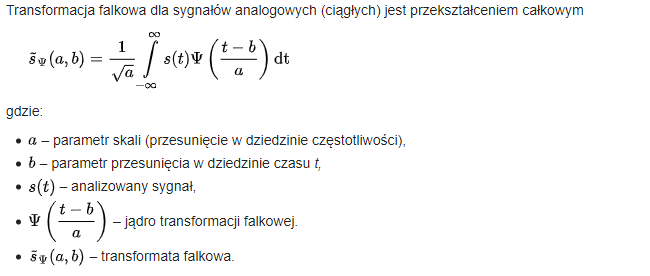
\includegraphics[width=0.8\textwidth]{falkowa.PNG}
	\caption{Definicja transformacji falkowej}
\end{figure}

Wynikiem transformacji falkowej są współczynniki, których wartości są zależna od parametrów a i b oraz sygnału s(t). Dla danych wartości a i b współczynnik jest miarą podobieństwa pomiędzy daną falką a wybranym fragmentem sygnału s(t).

\begin{figure}[ht]
	\centering
	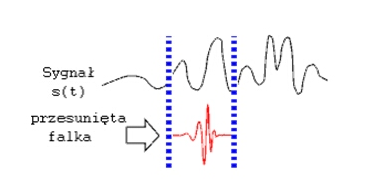
\includegraphics[width=0.8\textwidth]{wynik_falki.PNG}
	\caption{Wynik Transformacji Falkowej}
\end{figure}

\subsubsection{Transformacja Gabora}
Transformacja Gabora  jest szczególnym przypadkiem krótkotrwałej transformacji Fouriera. Służy do określania częstotliwości sinusoidalnej i zawartości fazowej lokalnych odcinków sygnału zmieniającego się w czasie. Funkcja do przekształcenia jest najpierw mnożona przez funkcję Gaussa, którą można uznać za funkcję okna, a wynikowa funkcja jest następnie przekształcana za pomocą transformaty Fouriera w celu uzyskania analizy czasowo-częstotliwościowej. Funkcja okna oznacza, że sygnał w pobliżu analizowanego czasu będzie miał większą wagę. 
Uzyskanie pełnego zestawu współczynników Gabora możliwe jest przy użyciu wzoru:\newline
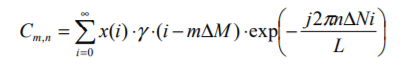
\includegraphics[width=0.4\textwidth]{transG1.png}

,gdzie: x(i) – analizowany sygnał, γ(i) – okno analizy, funkcja bi-ortogonalna do okna syntezy h(i), przy czym:\newline
	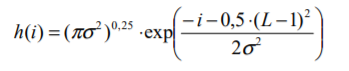
\includegraphics[width=0.4\textwidth]{transG2.png}

Analizowany sygnał x(i) może być przedstawiony jako suma:\newline
	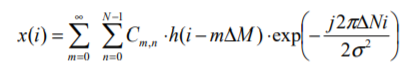
\includegraphics[width=0.4\textwidth]{transG3.png}

Transformacja Gabora jest przydatnym narzędziem w procesie przetwarzania i analizy sygnałów fonicznych. Jednak jej zastosowanie jest ograniczone ze względu na trudności z obliczaniem współczynników Cm,n oraz stałą szerokość okna analizy ograniczającą jej precyzję w dziedzinie czasu i częstotliwości.
\subsection{Analiza Cepstrum}
Analiza cepstrum jest nieliniową techniką przetwarzania sygnału o różnorodnych zastosowaniach w obszarach takich jak przetwarzanie mowy i obrazu.
Znane są dwie definicje cepstrum widma mocy C(τ):\newline
	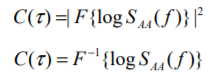
\includegraphics[width=0.28\textwidth]{Acepstrum1.png}

We wzorach SAA(f) reprezentuje dwuwstęgowe widmo mocy sygnału f(t), czyli SAA(f)=|F(f(t))|2. Porównując obie definicje można zauważyć, że jedna z nich wykorzystuje transformację Fouriera a druga transformację odwrotną. Jednak w wyniku obydwu przekształceń otrzymujemy reprezentację cepstralną przedstawiającą sygnał w dziedzinie czasu τ. Jest to dziedzina odpowiadająca odwrotności częstotliwości.
W przypadku sygnału cyfrowego cepstrum może być obliczone jako zestaw współczynników Cr na podstawie równania: \newline
	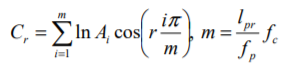
\includegraphics[width=0.3 \textwidth]{Acepstrum2.png}
gdzie: r - rząd współczynnika cepstralnego, lpr – liczba próbek w ramce, i – numer kolejnej próbki widma, Ai – amplituda i-tej próbki, fp – częstotliwość próbkowania, fc – maksymalna częstotliwość uwzględniona w analizie cepstralnej.


\subsection{Możliwość wykorzystania podanych metod według zadania projektowego}

\subsection{Narzędzia do analizy sygnałów cyfrowych}

\subsection{Wnioski}

\section{Koncepcja}
\label{sec:koncepcja}

\section{Implementacja}
\label{sec:implementacja}


\section{Uruchomienie}
\label{sec:uruchomienie}


\section{Podsumowanie}
\label{sec:podsumowanie}

\subsection{Tygodniowy harmonogram zadań}



\begin{tabular}{|p{2cm}|p{9cm}|p{3.5cm}|} \hline
Data & Zadanie & Osoba odpowiedzialna \\
\hline
16.03.2020 - 24.03.2020 & Lider zespołu, sporządzenie wniosków  i finalnej częsci raportu & Julia Borysławska \\
\hline
 & Zabranie informacji o Design Thinking'u (wady, zalety, metoda "Trzy fazy") & Sofiia Levchenko\\
\hline
& Zebranie informacji o Design Thinking'u (metody "Double Diamond" i "Pięć kroków") & Joanna Staleńczyk \\
\hline
& Zebranie informacji o narzędziach do obróbki tekstu & Jakub Tarczyński \\
\hline
& Zebranie informacji o narzędziach do organizacji pracy  & Jan Zobiów \\ 

\hline

\end{tabular}





\bibliographystyle{plabbrv} % plplain plabbrv plalpha
\begin{thebibliography}{SYCYfProjekt}
\bibitem{DesignThinking1}
 Visser, W. 2006, The cognitive artifacts of designing, Lawrence Erlbaum Associates.
\bibitem{DesignThinking2}
"Design Thinking: A Beginner’s Guide to the History, Terminologies and Methodologies" by Rhoda Sell \url{https://blog.prototypr.io/design-thinking-a-beginners-guide-to-the-history-terminologies-and-methodologies-e527f7afdcd1}
\bibitem{Proces1}
"The five steps of design thinking" by D.School, Stanford University’s Institute of Design \url{https://dschool-old.stanford.edu/sandbox/groups/designresources/wiki/36873/attachments/74b3d/ModeGuideBOOTCAMP2010L.pdf}
\bibitem{Proces2}
"The three overlapping phases of design thinking" by IDEO. \url{https://www.designkit.org/human-centered-design}
\bibitem{Proces3}
"The four-phased ‘Double Diamond’ process" by the Design Council \url{https://www.designcouncil.org.uk/news-opinion/what-framework-innovation-design-councils-evolved-double-diamond}
\end{thebibliography}

\end{document}
